\section{实证比较}
\sectionlead{section-4}{四、实证比较}{均值掩盖了哪些差别？依次看股票、投资者和交易事件。}

\subsection{4.1 股票与家庭}
\begin{frame}[label=slices]{同一批记录可以切成三种分析对象}
  \crumb{Part 4}{4.1 股票与家庭}{论文 V--VII}
  \small
  \begin{tabularx}{\linewidth}{@{}L{.24\linewidth}YY@{}}
    \toprule 一行是什么 & 字段示意 & 问题和方法\\\midrule
    股票 \(\times\) 月 & \(\underbrace{(j,m)}_{\text{股票、月份}}\ \mid\ \underbrace{A,L,D}_{\text{三项关注量}}\) &
      哪些股票受到更多关注？前 1,000 大 CRSP 股票的月面板回归。\\\midrule
    家庭 & \(\underbrace{i}_{\text{家庭}}\ \mid\ \underbrace{B_{i1},\ldots,B_{i,13}}_{\text{各主题列}}\ \mid\ S_i\) &
      哪些主题在同一家庭一起出现？加投机标的倾向 \(S_i\)，做 PCA。\\\midrule
    家庭 \(\times\) 股票 \(\times\) 订单 &
      \((i,j,e)\) 家庭、股票、订单\newline \((\tau,k)\) 相对时点、主题 &
      下单前何时研究、按何顺序？累积曲线与 Sankey。\\
    \bottomrule
  \end{tabularx}
  \finding{先看关注落在哪里，再看谁以相似方式研究，最后回到同股的订单时钟。}
\end{frame}

\begin{frame}[label=design]{股票月回归区分广度、用时和内容}
  \crumb{Part 4}{4.1 股票与家庭 · 股票月规格}{Table 4}
  \[
    Y_{jm}=\alpha+\beta z(\ln \mathrm{Cap}_{jm})+\gamma^\top Z_{jm}
               +\delta_{\mathrm{FF49}(j)}+\varepsilon_{jm},
    \qquad Y \in \{A,L,D\}.
  \]
  \small
  \begin{tabularx}{\linewidth}{@{}L{.25\linewidth}Y@{}}
    \toprule \(A\) 覆盖率 (1--3) & 股票月里做过该股研究的投资者比例（百分点）。\\
    \(L\) 总用时 (4) & \(\ln(1+\text{匹配到该股票月的总研究分钟})\)。\\
    \(D\) 内容倾斜 (5--6) & 查看价格图或技术的比例，减查看盈利、股利、其他基本面、分析师或官网的比例。\\\bottomrule
  \end{tabularx}
  \medskip
  {\small (1) 只放市值；(2) 加事件、股票特征与 FF49 行业项；(3) 再加可能内生的散户参与度。连续解释变量标准化。}
  \finding{3,962 个股票月，原表 Newey--West 月度滞后 2 阶。\(A\) 和 \(L\) 对应关注广度与总投入，\(D\) 看主题构成。}
  \scriptsize\jump{appendix-2}{A2 · 回归全表}
\end{frame}

\begin{frame}[label=size]{仅市值解释约三成的覆盖率变异}
  \crumb{Part 4}{4.1 股票与家庭 · 市值基准}{Table 4 (1)--(4)}
  \pair{
    \textbf{覆盖率 \(R^2\)}\par
    \begin{tikzpicture}[x=6.85cm,y=.69cm,font=\small]
      \foreach \y/\r/\id in {2/.315/{(1)},1/.447/{(2)},0/.484/{(3)}} {
        \fill[sampleblue!32] (0,\y) rectangle (\r,\y+.48);
        \node[anchor=west] at (0,\y+.24) {\id};
        \node[anchor=west] at (\r,\y+.24) {\r};}
    \end{tikzpicture}\par
    {\small (1) 市值；(2) 加基本特征与行业；(3) 加散户参与度。}}
  {\textbf{关注者比例的量级}\par\medskip
    {\fontsize{20}{22}\selectfont\bfseries\color{wine}1.01\% \(\to\) 2.04\%\par}
    {\small 市值（对数）提高 1 个标准差，覆盖率拟合值高 1.03 个百分点，\(t=14.42\)。}\par\medskip
    {\small 总用时规格的市值系数仍为正（0.49 对数点）。}}
  \finding{规模可能同时反映媒体曝光、流动性和熟悉度。接着看规模相近的股票之间还有哪些差别。}
\end{frame}

\newcommand{\coefrow}[5]{%
  \pgfmathsetmacro{\cihalf}{1.96*abs(#3/#4)}
  \node[anchor=east,inner sep=2pt] at (#2,#1) {#5};
  \draw[sampleblue,semithick] ({#3-\cihalf},#1)--({#3+\cihalf},#1);
  \fill[sampleblue] (#3,#1) circle[radius=1.52pt];}
\begin{frame}[label=adjusted]{控制规模后，财报与波动仍关联更多研究}
  \crumb{Part 4}{4.1 股票与家庭 · 控制后的比较}{Table 4 (2)--(4)}
  \begin{columns}[T,onlytextwidth]
    \column{.58\textwidth}\small
    \textbf{覆盖率 \(A\)，第 (2) 列（百分点）}\par
    \begin{tikzpicture}[x=5.5cm,y=.46cm,font=\scriptsize]
      \draw[quiet!45] (0,-.34)--(0,5.49);
      \coefrow{5}{-.39}{.30}{6.25}{财报月}
      \coefrow{4}{-.39}{.15}{4.92}{收益波动率}
      \coefrow{3}{-.39}{.10}{2.89}{CAPM beta}
      \coefrow{2}{-.39}{-.17}{-2.57}{ln 价格}
      \coefrow{1}{-.39}{-.07}{-2.10}{动量}
      \coefrow{0}{-.39}{-.23}{-2.95}{分红}
      \foreach \x in {-.3,0,.3} \node[below] at (\x,-.33) {\pgfmathprintnumber{\x}};
    \end{tikzpicture}\par
    {\scriptsize 线段据表内舍入系数和 \(t\) 值推算近似 95\% 区间。}
    \column{.39\textwidth}\small
    \textbf{总用时 \(L\)，第 (4) 列}\par
    财报月 \(+0.24\)、波动 \(+0.10\)、动量 \(+0.04\)（对数点）。\par\medskip
    动量在两列方向不同。总用时同时积累了看的人和他们的研究分钟。\par\medskip
    第 (3) 列另含散户参与度，其相关性作为描述。
  \end{columns}
  \finding{月度结果首先回答谁吸引关注。把时钟改到日频，能看到关注在事件前后的实际集中。}
\end{frame}

\begin{frame}[label=event]{财报、新品和并购附近出现日度关注尖峰}
  \crumb{Part 4}{4.1 股票与家庭 · 事件时间}{Figure 2 · 484 户}
  \begin{columns}[T,onlytextwidth]
    \column{.325\textwidth}\centering\small
     \textbf{A · Microsoft}\par
     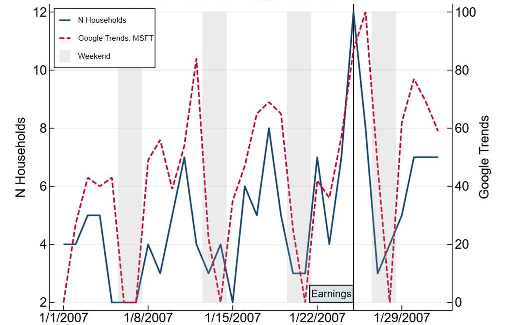
\includegraphics[width=\linewidth]{fig2a.pdf}\par 1/25 季度财报
    \column{.325\textwidth}\centering\small
     \textbf{B · Apple}\par
     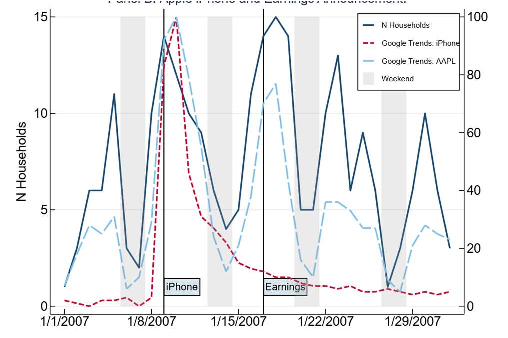
\includegraphics[width=\linewidth]{fig2b.pdf}\par 1/9 iPhone、1/17 财报
    \column{.325\textwidth}\centering\small
     \textbf{C · Sirius}\par
     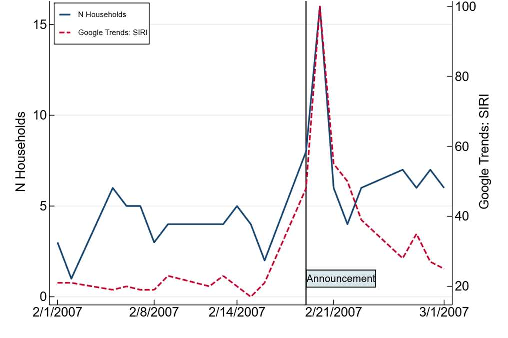
\includegraphics[width=\linewidth]{fig2c.pdf}\par 2/19 宣布与 XM 合并
  \end{columns}
  \medskip
  {\small 左轴为每日研究人数，右轴为标准化 Google Trends。各面板量程有别。}
  \finding{点击流与搜索在若干日期同步。Apple 的产品和股票峰值也显示，两种关注可被区分。}
\end{frame}

\begin{frame}[label=tilt]{股票特征对“看什么”的解释度较低}
  \crumb{Part 4}{4.1 股票与家庭 · 内容倾斜}{Table 4 (5)--(6)}
  \begin{columns}[T,onlytextwidth]
    \column{.61\textwidth}\small
    \textbf{价格覆盖率减基本面覆盖率，第 (6) 列}\par
    \begin{tikzpicture}[x=13cm,y=.52cm,font=\scriptsize]
      \draw[quiet!45] (0,-.33)--(0,3.44);
      \coefrow{3}{-.206}{.06}{4.63}{波动率}
      \coefrow{2}{-.206}{.05}{2.33}{动量}
      \coefrow{1}{-.206}{-.10}{-2.42}{分析师覆盖}
      \coefrow{0}{-.206}{.03}{.61}{市值（对数）}
      \foreach \x in {-.2,-.1,0,.1} \node[below] at (\x,-.34) {\pgfmathprintnumber{\x}};
    \end{tikzpicture}\par
    {\scriptsize 单位为百分点，线段为以原表系数和 \(t\) 值推算的近似区间。}
    \column{.36\textwidth}\small
    \textbf{对照覆盖率规格}\par
    \(R^2\)　0.079／0.090\par
    同样的扩展变量解释广度时，\(R^2=0.484\)。市值与倾斜的关联接近零且不精确。
  \end{columns}
  \finding{高波动、高动量的股票更偏价格研究。股票特征只解释了少部分主题差异，接下来比较投资者。}
\end{frame}

\begin{frame}[label=pc-why]{同一家庭的研究主题如何共同出现}
  \crumb{Part 4}{4.1 股票与家庭 · 换到投资者层}{VI · Table 5}
  \pair{\textbf{股票月回答}\par\small
    哪些股票更常被看，主题倾斜随什么变化？\par
    一行是股票和月份，\(Y\) 是覆盖、用时或倾斜。}
  {\textbf{家庭层回答}\par\small
    同一个人会一起看哪些主题？这些模式与所关注股票的类型是否同变？\par
    PCA 概括多列输入的主要变异方向。}
  \medskip
  \leadrow{交易频率只提供少量线索}{交易笔数与每笔研究分钟的 Pearson 相关为 \(-0.10\)，秩相关为 \(-0.22\)。}
  \finding{把主题参与和股票倾向并列放进同一家庭矩阵，可以区分研究范围与研究风格。}
\end{frame}

\begin{frame}[label=pc-input]{PCA 输入：主题参与与投机标的倾向}
  \crumb{Part 4}{4.1 股票与家庭 · 家庭矩阵}{VI · Table 5}
  \[
    B_{ik}=\mathbf{1}\{m_{ik}>2\},
    \qquad X_i=(B_{i1},\ldots,B_{i,13},S_i).
  \]
  \small
  \begin{tabularx}{\linewidth}{@{}L{.23\linewidth}YYY@{}}
    \toprule 行索引 & 价格图 & … 其他主题 & 投机标的倾向\\\midrule
    家庭 \(i\) & \(B_{i,\text{价格}}\) & \(B_{ik}\in\{0,1\}\) & \(S_i\in\mathbb R\)\\
    家庭 \(i'\) & \(B_{i',\text{价格}}\) & \(B_{i'k}\in\{0,1\}\) & \(S_{i'}\in\mathbb R\)\\\bottomrule
  \end{tabularx}\par\medskip
  \(m_{ik}\) 为每户每月在该主题的研究分钟，只计可匹配的股票。风险统计参与太少，13 个主题之外加一个连续 \(S_i\)。高分偏小、新、高波动、低价股；低分偏大、成熟、分红股。
  \finding{指标记录是否把主题纳入经常研究的范围，分钟数差异不会直接进入这些主题列。}
  \small\jump{appendix-6}{A6 · 表注与正文措辞}
\end{frame}

\newcommand{\loadingbar}[4]{%
  \node[anchor=east,inner sep=2pt] at (-.58,#1) {#2};
  \fill[#4!75] (0,#1-.18) rectangle (#3,#1+.18);
  \node[anchor=west,inner sep=2pt] at ({max(0,#3)},#1) {\pgfmathprintnumber[fixed,precision=2]{#3}};}
\begin{frame}[label=pc-one]{第一主成分刻画跨主题的共同参与}
  \crumb{Part 4}{4.1 股票与家庭 · PC1}{Table 5}
  \begin{columns}[T,onlytextwidth]
    \column{.63\textwidth}\centering
    \begin{tikzpicture}[x=6.7cm,y=.55cm,font=\small]
      \begin{scope}[xshift=2.3cm]
      \node[anchor=east,inner sep=2pt] at (0,6) {主题或股票倾向};
      \draw[quiet!30] (0,-.30)--(0,5.35);
      \foreach \y/\name/\v in {5/{未知新闻}/.36,4/{快照}/.32,3/{分析师}/.32,2/{价格图}/.31,1/{盈利}/.29,0/{投机标的倾向}/.01}{
        \node[anchor=east] at (0,\y) {\name};
        \fill[sampleblue!70] (0,\y-.17) rectangle (\v,\y+.17);
        \node[anchor=west] at (\v,\y) {\pgfmathprintnumber[fixed,precision=2]{\v}};}
      \end{scope}
    \end{tikzpicture}\par{\small 条长为载荷；选列展示。}
    \column{.35\textwidth}
    \greatnum{26.81\%}\par
    {\small 解释输入总变异\\特征值 3.75}\par\medskip
    {\small 13 项主题的载荷均为正，股票投机倾向近零。}
  \end{columns}
  \finding{PC1 较高的投资者通常同时参与更多主题。总分钟并非这一成分的直接输入。}
\end{frame}

\begin{frame}[label=pc-two]{第二主成分把快信息与投机标的联系起来}
  \crumb{Part 4}{4.1 股票与家庭 · PC2}{Table 5}
  \begin{columns}[T,onlytextwidth]
    \column{.67\textwidth}\centering
    \begin{tikzpicture}[x=4.6cm,y=.41cm,font=\scriptsize]
      \draw[quiet!55] (0,-.36)--(0,8.36);
      \loadingbar{8}{留言板}{.46}{wine}
      \loadingbar{7}{投机标的}{.43}{wine}
      \loadingbar{6}{综合快照}{.30}{wine}
      \loadingbar{5}{价格图}{.19}{wine}
      \loadingbar{4}{分析师}{0}{quiet}
      \loadingbar{3}{技术信号}{-.11}{sampleteal}
      \loadingbar{2}{其他基本面}{-.29}{sampleteal}
      \loadingbar{1}{盈利}{-.34}{sampleteal}
      \loadingbar{0}{股利}{-.47}{sampleteal}
    \end{tikzpicture}\par
    {\small 先读零线两侧，再看各条长短。选列载荷。}
    \column{.31\textwidth}
    \greatnum{8.77\%}\par
    {\small 解释输入总变异\\特征值 1.23}\par\medskip
    {\small 研究快信息与偏向投机标的在同一轴上。盈利、股利靠相反一侧。}
  \end{columns}
  \finding{这是主题与标的的联合变异。快慢两端也用于下文分组，不能用分组重新识别投机倾向的因果影响。}
\end{frame}

\subsection{4.2 交易时点与路径}
\begin{frame}[label=timing]{交易附近累积出较多同股研究}
  \crumb{Part 4}{4.2 交易时点与路径 · 研究何时发生}{Figure 3 · 50 户}
  {\centering
  \annotatedpanel{4.14cm}{fig3.pdf}{
    \draw[samplegold,line width=.75pt] (.382,.43) rectangle (.412,.68);
    \draw[samplegold,line width=.75pt] (.890,.16) rectangle (.922,.55);
  }\par}
  {\small 横轴：距本次交易的小时，\(0\) 为订单。纵轴：累计研究分钟。左侧均值与右侧中位数量程不同。}
  \finding{先读右图：约到交易前五天才见中位数累积，主要跳升临近下单；均值在更早时点也有累积。}
\end{frame}

\begin{frame}[label=path]{新的同股路径常在首个主题后结束}
  \crumb{Part 4}{4.2 交易时点与路径 · 主题之间的跳转}{Figure 4}
  \begin{columns}[T,onlytextwidth]
    \column{.61\textwidth}\centering
    \annotatedpanel{4.6cm}{fig4.pdf}{
       \draw[wine,line width=.55pt] (.01,.26) rectangle (.106,.91);
       \draw[wine,line width=.55pt] (.226,.118) rectangle (.319,.586);
       \draw[wine,line width=.55pt] (.907,.456) rectangle (.984,.517);
    }
    \column{.36\textwidth}\small
    \leadrow{入口}{快照、价格图、新闻较常见。}
    \leadrow{第二列 END}{最粗一支，表示首个主题后没有新增的计入主题。}
    \leadrow{右端 Further}{仍有更多出现的主题。}
    \medskip
    线宽为路径数，原路径的重复主题已删除。
  \end{columns}
  \finding{例：价格图 \(\to\) 盈利 \(\to\) 再看价格图，图上只留价格图 \(\to\) 盈利。484 户，16,930 个同股十天窗口。}
\end{frame}

\begin{frame}[label=buy-sell]{买卖之前，粗粒度主题路径相近}
  \crumb{Part 4}{4.2 交易时点与路径 · 按订单方向}{Figure 5 A/B}
  \pair{\centering\small\textbf{A · 买入}\par
    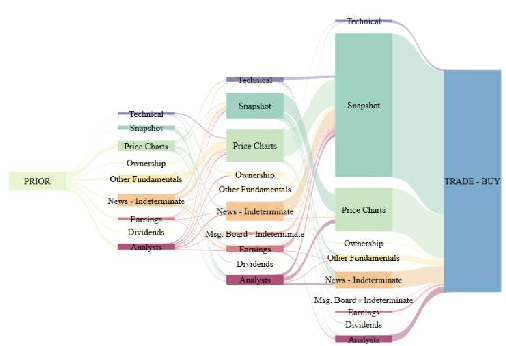
\includegraphics[width=\linewidth,height=3.88cm,keepaspectratio]{fig5a.pdf}\par}
  {\centering\small\textbf{B · 卖出}\par
    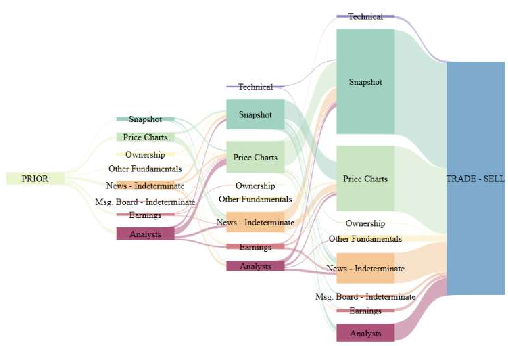
\includegraphics[width=\linewidth,height=3.88cm,keepaspectratio]{fig5b.pdf}\par}
  {\small 从右端买卖向左，回看同股之前十天的主题。线宽为路径数。}
  \finding{买卖前都常见快照和价格图。相似的是主题次序。}
\end{frame}

\begin{frame}[label=fast-slow]{按研究风格分组后，快信息组路径更窄}
  \crumb{Part 4}{4.2 交易时点与路径 · 按 PC2 分组}{Figure 5 C/D}
  \pair{\centering\small\textbf{C · 慢信息，PC2 最低五分位}\par
    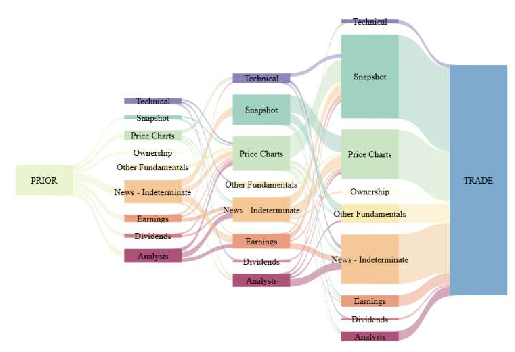
\includegraphics[width=\linewidth,height=3.88cm,keepaspectratio]{fig5c.pdf}\par}
  {\centering\small\textbf{D · 快信息，PC2 最高五分位}\par
    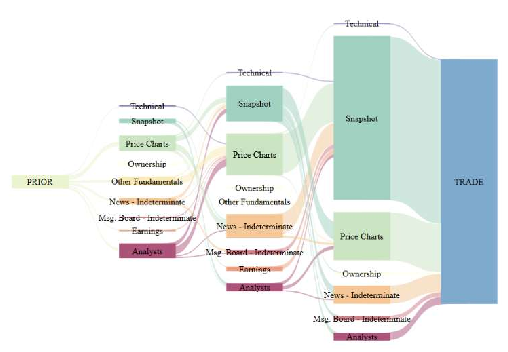
\includegraphics[width=\linewidth,height=3.88cm,keepaspectratio]{fig5d.pdf}\par}
  {\small 对照前两步：慢信息组路径更宽，快信息组常见快照或快照加价格图。}
  \finding{分组本身来自 PC2。接下来把主题分化及其他证据放回模型假设。}
\end{frame}
